\section{جداول}
\begin{frame}[fragile]{محیط حضور جدول}
\begin{latin}
\begin{lstlisting}[keywords={begin, end}, keywordstyle=\color{Mulberry}\textbf]
\begin{table}[h]
...
\end{table}
\end{lstlisting}
\end{latin}
\end{frame}

\begin{frame}[fragile]{محیط شکل‌دهی جدول}
\begin{latin}
\begin{lstlisting}[keywords={begin, end}, keywordstyle=\color{Mulberry}\textbf]
\begin{tabular}{<columns>}
<rows>
\end{tabular}
\end{lstlisting}
\end{latin}
\end{frame}

\begin{frame}{ستون‌ها}
\begin{itemize}\itemr
\item[-]
تراز افقی ستون‌های جدول‌‌ها در لاتک، در اولین آرگومان محیط‌ شکل‌دهی جداول تعیین می‌شوند.

\item[-]
ستون‌ها می‌توانند مقدار 
\lr{\texttt{r}}،
\lr{\texttt{c}}
و 
\lr{\texttt{l}}
داشته باشند که به ترتیب، راست‌چین، وسط‌چین و چپ‌چین می‌شوند.
\end{itemize}
\end{frame}

\begin{frame}[fragile]{نمونه کد}
\begin{latin}
\begin{lstlisting}[keywords={begin, end}, keywordstyle=\color{Mulberry}\textbf]
\begin{table}[h]
\begin{center}
\begin{tabular}{lcr}
I am left-aligned & 
I am at the center & 
I am right-aligned \\

left, in the second line &
2$^{\text{nd}}$ line, center placed &
enjoying the right side \\

\end{tabular}
\end{center}
\end{table}
\end{lstlisting}
\end{latin}
\end{frame}

\begin{frame}{خروجی}
\begin{center}
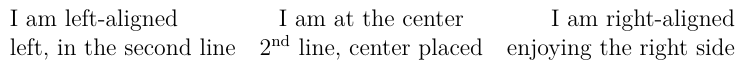
\includegraphics[width=\textwidth]{docs/images/simple-table}
\end{center}
\end{frame}

\begin{frame}{ستون‌ها}
\begin{itemize}\itemr
\item[-]
خط‌های جداکننده‌ی ستون‌ها در محل تعیین تراز ستون‌ها قرار می‌گیرند.
\end{itemize}
\end{frame}

\begin{frame}[fragile]{نمونه کد}
\begin{latin}
\begin{lstlisting}[keywords={begin, end}, keywordstyle=\color{Mulberry}\textbf]
\begin{table}[h]
\begin{center}
\begin{tabular}{l|c|r}   % HERE
I am left-aligned & 
I am at the center & 
I am right-aligned \\

left, in the second line &
2$^{\text{nd}}$ line, center placed &
enjoying the right side \\

\end{tabular}
\end{center}
\end{table}
\end{lstlisting}
\end{latin}
\end{frame}

\begin{frame}{خروجی}
\begin{center}
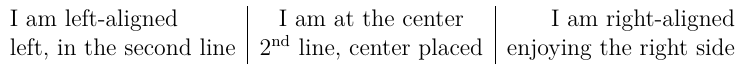
\includegraphics[width=\textwidth]{docs/images/1}
\end{center}
\end{frame}

\begin{frame}[fragile]{نمونه کد}
\begin{latin}
\begin{lstlisting}[keywords={begin, end}, keywordstyle=\color{Mulberry}\textbf]
\begin{table}[h]
\begin{center}
\begin{tabular}{|lcr|}   % HERE
I am left-aligned & 
I am at the center & 
I am right-aligned \\

left, in the second line &
2$^{\text{nd}}$ line, center placed &
enjoying the right side \\

\end{tabular}
\end{center}
\end{table}
\end{lstlisting}
\end{latin}
\end{frame}

\begin{frame}{خروجی}
\begin{center}
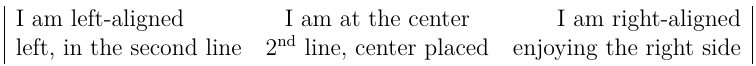
\includegraphics[width=\textwidth]{docs/images/2}
\end{center}
\end{frame}

\begin{frame}[fragile]{نمونه کد}
\begin{latin}
\begin{lstlisting}[keywords={begin, end}, keywordstyle=\color{Mulberry}\textbf]
\begin{table}[h]
\begin{center}
\begin{tabular}{|l|c|r|}   % HERE
I am left-aligned & 
I am at the center & 
I am right-aligned \\

left, in the second line &
2$^{\text{nd}}$ line, center placed &
enjoying the right side \\

\end{tabular}
\end{center}
\end{table}
\end{lstlisting}
\end{latin}
\end{frame}

\begin{frame}{خروجی}
\begin{center}
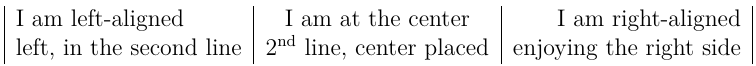
\includegraphics[width=\textwidth]{docs/images/3}
\end{center}
\end{frame}

\begin{frame}{ستون‌ها}
\begin{itemize}\itemr
\item[-]
ردیف‌‌های جدول در داخل محیط 
\lr{\texttt{tabular}}
نوشته می‌شوند.

\item[-]
هر ستون با علامت 
\lr{\texttt{\&}}
جدا می‌شود.

\item[-] 
هر ردیف با 
\textbackslash \textbackslash $\,$
از ردیف بعدی جدا می‌شود.

\item[-]
خطوط افقی با دستور 
\lr{\texttt{\textbackslash hline}}
ساخته می‌شوند.
\end{itemize}
\end{frame}

\begin{frame}[fragile]{نمونه کد}
\begin{latin}
\begin{lstlisting}[keywords={begin, end}, keywordstyle=\color{Mulberry}\textbf]
\begin{table}[h]
\begin{center}
\begin{tabular}{|l|c|r|}   
\hline   % HERE
I am left-aligned & 
I am at the center & 
I am right-aligned \\

left, in the second line &
2$^{\text{nd}}$ line, center placed &
enjoying the right side \\
\hline    % HERE
\end{tabular}
\end{center}
\end{table}
\end{lstlisting}
\end{latin}
\end{frame}

\begin{frame}{خروجی}
\begin{center}
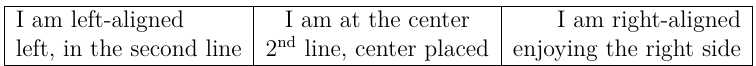
\includegraphics[width=\textwidth]{docs/images/flhline}
\end{center}
\end{frame}

\begin{frame}[fragile]{نمونه کد}
\begin{latin}
\begin{lstlisting}[keywords={begin, end}, keywordstyle=\color{Mulberry}\textbf]
\begin{table}[h]
\begin{center}
\begin{tabular}{|l|c|r|}   
\hline   % HERE
I am left-aligned & 
I am at the center & 
I am right-aligned \\
\hline   % HERE
left, in the second line &
2$^{\text{nd}}$ line, center placed &
enjoying the right side \\
\hline    % HERE
\end{tabular}
\end{center}
\end{table}
\end{lstlisting}
\end{latin}
\end{frame}

\begin{frame}{خروجی}
\begin{center}
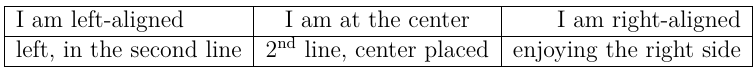
\includegraphics[width=\textwidth]{docs/images/fmlhline}
\end{center}
\end{frame}

\begin{frame}[fragile]{نمونه کد}
\begin{latin}
\begin{lstlisting}[keywords={begin, end}, keywordstyle=\color{Mulberry}\textbf]
\begin{table}[h]
\begin{center}
\begin{tabular}{|l|c|r|}   
\hline   % HERE
I am left-aligned & I am at the center & I am right-aligned \\
\hline   % HERE
\hline   % HERE
left, in the second line &
2$^{\text{nd}}$ line, center placed &
enjoying the right side \\
\hline    % HERE
some text & another text & last text \\
\hline    % HERE
\end{tabular}
\end{center}
\end{table}
\end{lstlisting}
\end{latin}
\end{frame}

\begin{frame}{خروجی}
\begin{center}
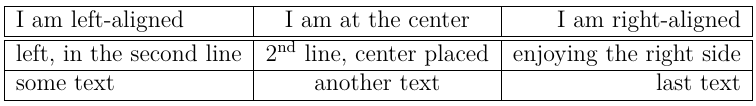
\includegraphics[width=\textwidth]{docs/images/twohline}
\end{center}
\end{frame}
